\documentclass[journal]{IEEEtran}

\usepackage[T1]{fontenc}
\usepackage{amsmath,amssymb,mathtools}
\usepackage{graphicx}
\usepackage{booktabs,tabularx,array,multirow}
\usepackage{siunitx}
\usepackage{enumitem}
\usepackage{xcolor}
\usepackage{tikz}
\usetikzlibrary{positioning,arrows.meta,fit,backgrounds,calc}
\usepackage{cite}
\usepackage{url}
\usepackage{hyperref}
\usepackage{microtype}

\hypersetup{
  colorlinks=true,
  linkcolor=blue,
  citecolor=blue,
  urlcolor=blue
}
\sisetup{detect-all,per-mode=symbol}

\newcommand{\todo}[1]{\textcolor{red}{\textbf{[TO BE UPDATED: #1]}}}
\newcommand{\softrobotagent}{\textsc{Softrobot-Agent}}
\newcommand{\MainAgent}{\textsc{Main}}
\newcommand{\Reporter}{\textsc{Reporter}}
\newcommand{\MuJoCo}{MuJoCo}
\newcommand{\GVS}{GVS}
\newcommand{\Vtask}{V_{\tau}}
\newcommand{\Rset}{\mathcal{R}}
\newcommand{\dd}{\mathrm{d}}
\newcolumntype{Y}{>{\raggedright\arraybackslash}X}

\title{Softrobot-Agent: Physics-Guided Mathematical Research for Autonomous Soft-Robot Design and Control}

\author{Anonymous Authors%
\thanks{Working manuscript. Author information, affiliations, and target venue will be added after the technical content and experimental comparisons are finalized.}}

\begin{document}
\maketitle

\begin{abstract}
Designing tendon-driven soft robots requires more than searching geometric and material parameters. A researcher must identify the physical mechanism limiting a task, decide which structural or control variables are relevant, formulate an appropriate mathematical investigation, and revise the design when new evidence changes the working hypothesis. This paper presents \softrobotagent{}, a research-oriented framework that organizes these activities into a physics-grounded agentic process. Its method combines adaptive physical-hypothesis formation, task-conditioned composable mathematical research, and evidence-guided structure--control refinement. A parameterized physical research problem connects registered design parameters and observables to task constraints and an appropriate inner equilibrium, dynamics, or control problem. The mathematical layer distinguishes four sensitivity semantics: mechanism-level (M0), fixed-input physical (M1), re-optimized task-capability (M2), and closed-loop (M3). Deterministic software performs problem compilation, differentiation routing, numerical analysis, and validity checks; the agent selects the scientific question and decides how to act on the resulting evidence. We evaluate the framework on eleven completed tendon-driven robot studies spanning active reach, tracking, orientation, loading, contact, impact recovery, and passive structural response. The archived portfolio contains 30 passed required conditions across 32 required/control records; two additional frozen control conditions in the impact-recovery study are reported separately. A nine-segment, four-tendon passive-design case provides a detailed mechanism-design study, while a separate local sensitivity audit reports 18 task-metric derivative pairs with a maximum relative discrepancy of 0.1191\% between KKT-based implicit sensitivities and re-equilibration finite differences. Matched comparisons against LLM-only design and direct bottom-level mathematical-tool use are being conducted and will be incorporated after completion.
\end{abstract}

\begin{IEEEkeywords}
Soft robotics, continuum robots, tendon-driven robots, robot co-design, scientific agents, mathematical research, sensitivity analysis, physical reasoning.
\end{IEEEkeywords}

\section{Introduction}
\label{sec:introduction}

\subsection{Robot co-design as a scientific research problem}

Tendon-driven soft robots exhibit strong coupling among morphology, material properties, tendon routing, unilateral constraints, and actuation. Segment lengths and cross-sections affect elastic response; tendon offsets and guide locations determine force-transmission geometry; payout and assembly conditions determine when tendons become slack or taut; and the resulting structure constrains the control actions that can be realized. Consequently, a design change can alter several physical mechanisms at once.

When a robot fails a task, the next useful action is not necessarily another parameter update. The limiting factor may be insufficient structural capability, an unsuitable control sequence, an active-set transition, an inaccurate reduced model, or an interaction among several effects. A researcher may need to inspect an equilibrium, compare fixed-input responses, estimate a sensitivity, test a competing physical explanation, or replace the mathematical formulation being used. The challenge is therefore not only to optimize a given design problem, but also to determine which problem should be investigated next.

Numerical optimization is effective when the objective, decision variables, constraints, and model have already been specified. It does not generally determine whether those choices capture the physical mechanism currently limiting the robot. Conversely, an LLM can propose geometries, interpret simulation outcomes, and suggest design changes, but an unstructured language-model loop does not by itself guarantee that a physical hypothesis has been translated into a well-defined mathematical problem or that a proposed modification is supported by quantitative evidence.

We therefore treat autonomous soft-robot co-design as an iterative scientific process. The agent should be able to interpret task and physical observations, formulate a testable mechanism hypothesis, choose an appropriate mathematical or physical investigation, and revise its research direction when the evidence does not support the expected behavior. This process is related to the abductive--deductive--empirical cycle of scientific reasoning: abduction proposes a plausible explanation, deduction derives testable consequences, and investigation evaluates those consequences \cite{peirce1878}.

\subsection{Research question}

The central question of this work is:

\begin{quote}
How can an LLM agent use mathematical and physical evidence to autonomously investigate and improve soft-robot structure and control, rather than relying only on direct design generation or unguided candidate search?
\end{quote}

This question has two connected parts. First, how can an agent determine which physical mechanism, design parameter, or control variable is worth investigating? Second, how can the resulting mathematical and physical evidence change the subsequent research action, including the possibility of changing the parameterization, mathematical method, structure, or control strategy?

\subsection{Methodological overview}

We introduce \softrobotagent{}, a research-oriented framework for tendon-driven soft-robot design and control. The framework is organized around three coupled capabilities.

\paragraph{C1: Mechanism-guided adaptive research.}
The agent interprets physical observations as evidence for or against explicit hypotheses. It identifies expected and weakening observations, selects diagnostic or design actions, and can revise its research route when intermediate results invalidate the current explanation. The contribution is not simply choosing a parameter to optimize; it is deciding which physical relationship should be investigated and when the current research question should change.

\paragraph{C2: Task-conditioned composable mathematical research.}
A high-level research intent is represented as a parameterized physical research problem. The problem combines a frozen task contract, registered design parameters, physical observables, an inner equilibrium/dynamics/control problem, and a requested sensitivity or optimization semantics. Reusable mathematical operations are then selected and executed with explicit input requirements, numerical validity checks, and evidence outputs.

\paragraph{C3: Cross-task evidence-grounded research continuity.}
Knowledge, mathematical results, candidate designs, physical observations, and execution traces are organized so that later decisions can reuse earlier findings without treating them as universally valid. A deterministic evidence layer preserves numerical facts, while a read-only reporter explains their physical implications and limitations. A hierarchical context representation exposes decision-relevant summaries and keeps detailed numerical records available on demand.

These capabilities are supported by an executable research harness and a multi-task evaluation suite. The paper does not claim new KKT, envelope-theorem, implicit-differentiation, or finite-difference theorems. Its methodological contribution is to organize established mathematical tools and scientific-reasoning principles into an agent-directed process with explicit problem semantics and evidence boundaries.

\subsection{Evaluation overview}

The completed study portfolio contains eleven task cases, T01--T10 and PHS-2D, covering active reach-and-hold, loaded response, fast motion, trajectory tracking, tool-axis orientation, timed scanning, shared-structure multi-task design, passive progressive stiffness, contact interaction, impact recovery, and passive tendon-constrained response. Across the archived task summary, 30 required conditions passed; two additional frozen control conditions in T10 are reported separately and did not pass the full recovery criteria. These are completed-case results, not multi-seed success-rate estimates.

A nine-segment, four-tendon PHS-2D study is used as the principal passive mechanism-design case. Its mathematical evidence is complemented by a local sensitivity audit that compares KKT-based implicit task-metric derivatives with finite differences obtained by rebuilding the perturbed design and re-solving equilibrium. A matched comparison among LLM-only design, direct bottom-level mathematical-tool use, and the complete \softrobotagent{} method is being conducted on four representative tasks. No comparative outcome is claimed before those runs are complete.

\subsection{Paper organization}

Section~\ref{sec:formulation} defines the design, task, and research-state formulations. Section~\ref{sec:method} presents the research method and its multi-level sensitivity semantics. Section~\ref{sec:implementation} describes the executable system. Sections~\ref{sec:experimental-setup}--\ref{sec:results} report the completed task portfolio and the current mathematical evidence. Section~\ref{sec:hardware} reserves a separate place for physical-robot demonstrations. The final sections discuss interpretation, scope, and future work.

\section{Related Work}
\label{sec:related}

\subsection{Tendon-driven continuum robots and morphology--control co-design}

Continuum robots have been studied using constant-curvature models, Cosserat-rod formulations, and other reduced-order or geometrically exact representations. Reviews of continuum-robot design and kinematic modeling emphasize the relationship between geometry, actuation, and achievable motion \cite{webster2010design}. General tendon-routing formulations provide a basis for analyzing statics and dynamics under external loading \cite{rucker2011computing}. In tendon-driven systems, the design problem is further complicated by tension-only actuation, tendon slackness, routing geometry, and changes in the active set of unilateral constraints.

Soft-robot co-design benchmarks provide reusable environments for evaluating morphology and control. Evolution Gym studies large-scale evolution of soft-robot bodies and controllers \cite{bhatia2022evolutiongym}; SoftZoo investigates co-design across diverse locomotion environments \cite{wang2023softzoo}; and SoMoGym provides tools for developing and evaluating soft-robot controllers \cite{graule2022somogym}. These works establish the importance of reusable design spaces and task-level evaluation. Our focus is complementary: we study how a research agent identifies the physical question that should be investigated and organizes mathematical evidence to guide structure and control refinement.

\subsection{Foundation models for robot design and scientific workflows}

Recent work has explored foundation models for soft-robot design and co-design. RoboCrafter-QA studies foundation-model-based evaluation and generation of soft-robot designs \cite{chen2026robocrafter}, while Debate2Create uses multi-agent debate and physics-based evaluation for robot co-design \cite{qiu2026debate2create}. These studies demonstrate the potential of language-model reasoning for design generation and iterative candidate refinement.

Scientific-agent evaluation has also emphasized the need to assess workflow execution and evidence quality rather than relying only on plausible language outputs. ScienceAgentBench provides a benchmark for evaluating language agents on data-driven scientific discovery tasks \cite{chen2025scienceagentbench}. Our work focuses on the physical and mathematical research loop in tendon-driven robots: how an agent forms a physical hypothesis, constructs a parameterized mathematical question, and changes its subsequent research action in response to evidence.

\subsection{Sensitivity analysis and differentiable optimization}

KKT conditions and Lagrange multipliers provide local optimality and active-constraint information for constrained optimization \cite{boyd2004convex,nocedal2006numerical}. Perturbation analysis studies how optimal solutions and optimal values change as problem parameters vary \cite{bonnans2000perturbation}. Under appropriate regularity and optimality conditions, the envelope theorem relates the sensitivity of an optimized value to partial derivatives of the Lagrangian. Differentiable optimization layers have demonstrated how selected optimization problems can be embedded in differentiable computation graphs \cite{amos2017optnet}.

These mathematical tools are not universally applicable to robot-design parameters. Rebuilding a simulator model, switching a tendon active set, changing a discrete topology, or encountering contact may require implicit differentiation, controlled finite differences, directional analysis, or an explicit declaration that an ordinary derivative is unavailable. We use these established methods as composable research operations and make their assumptions and scope explicit.

\subsection{Scientific reasoning, evidence, and active diagnosis}

Scientific reasoning involves proposing explanations, deriving consequences, and evaluating them against observations. The abductive role of hypothesis formation is classically distinguished from deduction and induction \cite{peirce1878}. Experimental-design theory studies how to select observations or interventions under uncertainty and cost \cite{chaloner1995bayesian}. In our setting, the agent proposes physical explanations and discriminating observations, while deterministic tools execute the requested analysis and preserve the resulting evidence. The current system does not claim calibrated Bayesian information gain or numerical value-of-information optimization; it uses explicit expected and weakening observations, evidence scope, and computational cost to support research decisions.

\subsection{Positioning}

The proposed framework does not claim that morphology--control co-design, sensitivity analysis, implicit differentiation, or LLM-based design generation is new in isolation. Its focus is the organization of these capabilities into a task-conditioned research process: the agent chooses the scientific question and relevant parameter/observable groups; deterministic software constructs and validates the mathematical problem; numerical analysis produces scoped evidence; and the agent uses that evidence to refine the structure, control, or research route.

\section{Research Formulation}
\label{sec:formulation}

\subsection{Robot design and task contracts}

Let a robot design be represented by
\begin{equation}
d=(d_{\mathrm{top}},d_{\mathrm{geom}},d_{\mathrm{mat}},
d_{\mathrm{route}},d_{\mathrm{assembly}},d_{\mathrm{act}}),
\label{eq:design}
\end{equation}
where the components describe topology, geometry, material properties, tendon routing, assembly and payout parameters, and actuation-related parameters. Continuous variables may include segment lengths, cross-section dimensions, Young's modulus, tendon offsets, and guide locations. Discrete variables include segment count, tendon count, and routing topology.

An active task uses a finite-horizon control sequence
\begin{equation}
U=(u_0,u_1,\ldots,u_{N-1}),
\end{equation}
where each $u_k$ may represent tendon tensions or another registered input. A passive fixed-payout task has no commanded control sequence; its response is determined by the structure, unilateral tendon constraints, initial condition, and external loading.

A task $\tau$ is represented by a frozen contract containing its targets, initial state, loading conditions, time horizon, observables, units, thresholds, sampling semantics, and evaluation rules. It induces normalized constraint functions
\begin{equation}
g_{\tau,i}(d,U)\leq 0,\qquad i=1,\ldots,m_\tau.
\label{eq:taskconstraints}
\end{equation}
A non-positive value denotes satisfaction of the corresponding constraint. The LLM may interpret task intent and select which registered physical quantities are scientifically relevant, but it cannot silently modify the task's acceptance thresholds, coordinate frames, units, or sampling rules.

For a reach-and-hold task, representative constraints include
\begin{align}
g_{\mathrm{terminal}} &=
\frac{\|p(T;d,U)-p^\star\|}{\epsilon_p}-1,\\
g_{\mathrm{hold,pos},k} &=
\frac{\|p(t_k;d,U)-p^\star\|}{\epsilon_p}-1,\\
g_{\mathrm{hold,vel},k} &=
\frac{\|v(t_k;d,U)\|}{\epsilon_v}-1.
\end{align}
For tracking, a corresponding constraint may be
\begin{equation}
g_{\mathrm{track},k}=
\frac{\|p(t_k;d,U)-r(t_k)\|}{\epsilon_{\mathrm{track}}}-1,
\end{equation}
where the tolerance and sample times come from the frozen tracking contract.

\subsection{Task-conditioned design capability}

For an active task, define the best achievable normalized violation for a fixed structure:
\begin{equation}
V_\tau(d)=
\inf_{U\in\mathcal U(d)}
\max_{i=1,\ldots,m_\tau}g_{\tau,i}(d,U),
\label{eq:capability}
\end{equation}
where $\mathcal U(d)$ is the admissible control set. If the global optimum is attained, $V_\tau(d)\leq0$ indicates that a feasible input sequence exists in the specified model. In nonconvex numerical problems, a solver typically returns a best-found value rather than a certified global optimum; failure to find a feasible sequence is therefore not proof of infeasibility.

For a family of task conditions $\mathcal T$ sharing one structure but allowing condition-specific controls,
\begin{equation}
V_{\mathcal T}(d)=
\inf_{\{U_c\}_{c\in\mathcal T}}
\max_{c\in\mathcal T,\,i}
g_{c,i}(d,U_c).
\label{eq:multi-capability}
\end{equation}
This formulation measures the worst task capability of one shared structure rather than the performance of separately tailored morphologies.

\subsection{Research as a sequential decision process}

At research step $k$, define the state
\begin{equation}
s_k=(\tau,d_k,\mathcal H_k,\mathcal E_k,\mathcal B_k),
\label{eq:researchstate}
\end{equation}
where $\mathcal H_k$ is the set of active physical hypotheses, $\mathcal E_k$ is the accumulated evidence, and $\mathcal B_k$ is the remaining resource budget. The agent selects a research action
\begin{equation}
a_k\in\mathcal A_{\mathrm{adm}}(s_k),
\end{equation}
which may include a mathematical inspection, sensitivity analysis, interaction study, structural modification, control optimization, physical experiment, or evidence review. The resulting observation $y_k$ updates the research state:
\begin{equation}
(\mathcal H_{k+1},\mathcal E_{k+1},d_{k+1})
=\Phi(s_k,a_k,y_k).
\label{eq:researchupdate}
\end{equation}
An action need not improve the design immediately. It may instead reject a hypothesis, reveal that a mathematical method is inapplicable, or motivate a different parameterization.

The objective is to improve task-relevant design capability while producing interpretable and reusable evidence under bounded computational resources. This motivates evaluating both physical performance and the quality of the research decisions that lead to it.

\section{Method: Physics-Guided Agentic Research}
\label{sec:method}

\subsection{Overview}

\softrobotagent{} organizes robot co-design as an adaptive research loop rather than a fixed sequence of optimizer calls. The agent first interprets the task and available physical observations, proposes a mechanism hypothesis, and chooses a research question. A deterministic mathematical layer turns that question into a typed parameterized physical problem, selects an applicable numerical method, and returns validated evidence. The agent then decides whether to refine the current design, change the parameter group, investigate a different mechanism, revise the control formulation, or perform an independent physical evaluation.

Fig.~\ref{fig:research-framework} summarizes the division of responsibility. The agent owns the scientific choice; fixed software owns task semantics, parameter resolution, numerical execution, and evidence integrity. The \Reporter{} provides a read-only physical interpretation of completed evidence, while the \MainAgent{} retains the final research decision.

\begin{figure*}[t]
\centering
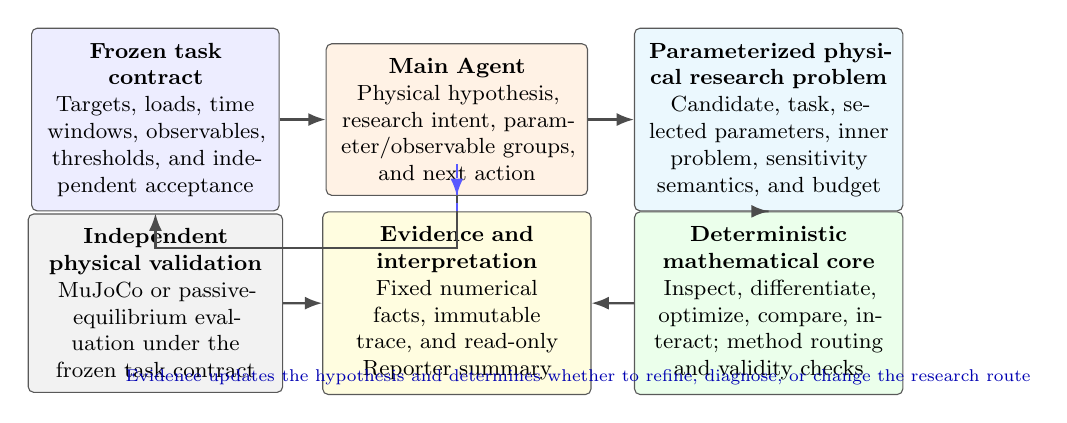
\begin{tikzpicture}[
  scale=0.88, transform shape,
  node distance=1.0cm and 1.05cm,
  base/.style={draw=black!65, rounded corners=2pt, align=center,
               minimum height=1.45cm, text width=3.15cm,
               font=\small, inner sep=6pt},
  task/.style={base, fill=blue!7},
  agent/.style={base, fill=orange!10, text width=3.35cm},
  problem/.style={base, fill=cyan!8, text width=3.45cm},
  math/.style={base, fill=green!8, text width=3.45cm},
  evidence/.style={base, fill=yellow!12, text width=3.45cm},
  physical/.style={base, fill=gray!10, text width=3.25cm},
  arrow/.style={-{Latex[length=2.2mm]}, thick, draw=black!70},
  feedback/.style={-{Latex[length=2.2mm]}, thick, dashed, draw=blue!65}
]
\node[task] (task) at (0,0) {\textbf{Frozen task contract}\\Targets, loads, time windows, observables, thresholds, and independent acceptance};
\node[agent] (agent) at (4.35,0) {\textbf{Main Agent}\\Physical hypothesis, research intent, parameter/observable groups, and next action};
\node[problem] (problem) at (8.85,0) {\textbf{Parameterized physical research problem}\\Candidate, task, selected parameters, inner problem, sensitivity semantics, and budget};
\node[math] (math) at (8.85,-2.65) {\textbf{Deterministic mathematical core}\\Inspect, differentiate, optimize, compare, interact; method routing and validity checks};
\node[evidence] (evidence) at (4.35,-2.65) {\textbf{Evidence and interpretation}\\Fixed numerical facts, immutable trace, and read-only Reporter summary};
\node[physical] (physical) at (0,-2.65) {\textbf{Independent physical validation}\\MuJoCo or passive-equilibrium evaluation under the frozen task contract};

\draw[arrow] (task) -- (agent);
\draw[arrow] (agent) -- (problem);
\draw[arrow] (problem) -- (math);
\draw[arrow] (math) -- (evidence);
\draw[arrow] (agent.south) -- ++(0,-0.75) -| (physical.north);
\draw[arrow] (physical) -- (evidence);
\draw[feedback] (evidence.north) -- ++(0,0.7) -| (agent.south);
\node[font=\scriptsize, text=blue!70!black, align=center] at (6.1,-3.72) {Evidence updates the hypothesis and determines whether to refine, diagnose, or change the research route};
\end{tikzpicture}

\caption{Physics-guided agentic research loop. The \MainAgent{} selects the physical hypothesis, parameter/observable groups, and research action. Fixed software compiles and validates the parameterized physical research problem, executes the appropriate mathematical operation, and preserves numerical evidence. The \Reporter{} summarizes physical implications and limitations; the agent then chooses the next design or research action.}
\label{fig:research-framework}
\end{figure*}

The sensitivity capability is available from the beginning of a study, but it is not a mandatory stage in every iteration. Before an initial candidate exists, the agent may formulate a structural mechanism hypothesis and select a candidate design. Once a candidate and working point are available, the mathematical layer can calculate local sensitivities. If the current topology is discrete, the response is non-smooth, or a mechanism hypothesis is already sufficiently specific, the agent may instead choose a direct structural or physical test.

\subsection{Research intent and parameterized physical research problems}

A high-level research request is represented by a parameterized physical research problem (PPRP):
\begin{equation}
\mathcal P_k =
(\tau,d_k,\mathcal D_k,\mathcal O_k,\mathcal F_k,
\sigma_k,\mathcal B_k),
\label{eq:pprp}
\end{equation}
where $\tau$ is the frozen task contract, $d_k$ is the current candidate, $\mathcal D_k$ is the selected parameter group, $\mathcal O_k$ is the selected set of physical observables, $\mathcal F_k$ specifies the inner physical problem, $\sigma_k$ is the requested analysis semantics, and $\mathcal B_k$ is the allocated mathematical budget.

The agent supplies the scientific content of the request: the working hypothesis, the parameter group worth investigating, the physical quantities that could reveal the proposed mechanism, and whether the comparison should hold the input fixed, re-optimize control, or evaluate a closed-loop controller. The fixed program resolves these choices against registered capabilities. It binds parameter paths and units, compiles task constraints from the frozen contract, checks whether the requested observables exist, selects the inner solver, and constructs the numerical request. The agent does not manually assemble Jacobian matrices, choose finite-difference step sizes, or manipulate solver-specific KKT arrays.

This separation makes the mathematical interface composable without allowing the language model to invent unregistered physical quantities or silently change task acceptance criteria. A proposed mechanism indicator must be built from registered observables and pass dimensional and applicability checks before it can be used as an optimization objective.

\subsection{Two dimensions of sensitivity organization}

The mathematical research layer organizes sensitivity along two independent dimensions.

\paragraph{Parameter dimension.}
The parameter registry describes what each design variable changes and which analysis routes can use it. Representative groups include:
\begin{itemize}[leftmargin=*]
  \item \textbf{Geometry:} segment length, cross-section, wall thickness, and guide location;
  \item \textbf{Material:} Young's modulus, density, damping, and other constitutive parameters;
  \item \textbf{Tendon routing:} offset, radius, angle, anchor position, and path geometry;
  \item \textbf{Assembly and actuation:} fixed payout, pretension, tension bounds, and actuator limits;
  \item \textbf{Controller:} NMPC weights, feedback gains, and other controller parameters;
  \item \textbf{Discrete morphology:} segment count, tendon count, routing topology, and cross-section type.
\end{itemize}
Continuous parameters may support derivatives or controlled perturbations. Discrete morphology changes are handled by candidate comparison rather than by assigning an ordinary continuous derivative.

\paragraph{Sensitivity semantics.}
For a selected parameter $d_j$, the agent must specify what output is being differentiated. We define four complementary levels.

\begin{table*}[t]
\centering
\caption{Task-conditioned multi-level sensitivity semantics. These are different mathematical objects, not four sequential optimizers.}
\label{tab:sensitivity-levels}
\small
\begin{tabularx}{\textwidth}{@{}l l Y Y@{}}
\toprule
Level & Mathematical object & Research question & Primary use \\
\midrule
M0: Mechanism & $\partial m(d)/\partial d_j$ &
How does a design parameter change a selected physical mechanism or geometric relation? &
Propose physically interpretable structural directions. \\
M1: Fixed-input physical response & $\left.\partial g_\tau(d,U)/\partial d_j\right|_U$ &
What changes when the structure is perturbed while the same input is replayed? &
Explain the physical effect of a structural modification under a controlled input. \\
M2: Re-optimized task capability & $\mathrm d V_\tau(d)/\mathrm d d_j$ &
How does task capability change when the structure is modified and the admissible control is re-optimized? &
Evaluate structure--control trade-offs and identify promising morphology changes. \\
M3: Closed-loop performance & $\partial g_{\tau,H}(d,\theta)/\partial z_j$ &
How does a structure or controller parameter affect the complete closed-loop execution? &
Assess controller-dependent behavior and high-fidelity task performance. \\
\bottomrule
\end{tabularx}
\end{table*}

The levels answer different questions and need not be executed in the order M0--M3. M0 can identify a mechanism worth shaping; M2 can test whether the mechanism direction improves the best task capability after control re-optimization. M1 explains the effect of a structural change under a fixed input. M3 evaluates the controller and high-fidelity execution path. A parameter can have different, or even opposing, effects under these different treatments.

For example, a tendon-routing change may improve a geometric decoupling metric at M0, worsen the response under a previously fixed tension sequence at M1, yet improve the best achievable task violation after the tension sequence is re-optimized at M2. The interpretation must retain the sensitivity semantics and control treatment.

\subsection{Mechanism-level analysis (M0)}

M0 starts from a physical hypothesis expressed in terms of registered observables. For a tendon-constrained mechanism, let $J_\ell(d)$ denote the Jacobian of tendon lengths with respect to generalized coordinates, and let $Z(d)$ span the local null space of the active tendon constraints. If the desired mechanism is to constrain tip motion while retaining motion in a selected middle region, one possible mechanism indicator is
\begin{equation}
m(d)=\|J_{\mathrm{tip}}(d)Z(d)\|_F^2,
\label{eq:m0-indicator}
\end{equation}
possibly combined with a term that prevents the middle-region response from collapsing. The agent may propose this relationship; the fixed program computes the registered Jacobians, constructs the indicator, checks its dimensions, and evaluates its sensitivity with respect to the selected continuous parameters.

The indicator is a mechanism proxy. A reduction in \eqref{eq:m0-indicator} does not by itself prove that finite-load passive stability or the original task has improved. It therefore motivates a subsequent equilibrium or task-capability evaluation rather than replacing it.

\subsection{Fixed-input and task-capability sensitivities (M1--M2)}

For M1, a previously defined input $U$ is held fixed:
\begin{equation}
S^{\mathrm{M1}}_{\tau,ij}
=
\left.\frac{\partial g_{\tau,i}(d,U)}{\partial d_j}\right|_U.
\label{eq:m1}
\end{equation}
This isolates the effect of changing the structure under the same actuation. It is useful for diagnosing the physical response, but it is not the final structure--control co-design objective.

For M2, the structure is perturbed and control is re-optimized through \eqref{eq:capability}. Introducing an epigraph variable $\rho$ gives
\begin{equation}
\begin{aligned}
\min_{U,\rho}\quad & \rho\\
\mathrm{s.t.}\quad&
g_{\tau,i}(d,U)-\rho\leq0,\quad \forall i,\\
&\ell_j(d)-U_j\leq0,\quad
U_j-h_j(d)\leq0,\quad \forall j.
\end{aligned}
\label{eq:epigraph}
\end{equation}
Let $\lambda_i\geq0$, $\alpha_j\geq0$, and $\beta_j\geq0$ denote multipliers for the task, lower-input, and upper-input constraints. Under local optimality, differentiability, an appropriate constraint qualification, and regularity of the optimizer, the envelope relation gives
\begin{equation}
\frac{\partial V_\tau}{\partial d_j}
=
\sum_i\lambda_i^\star
\frac{\partial g_{\tau,i}}{\partial d_j}
+
\sum_{\ell}\alpha_\ell^\star\frac{\partial \ell_\ell}{\partial d_j}
-
\sum_{\ell}\beta_\ell^\star\frac{\partial h_\ell}{\partial d_j}.
\label{eq:envelope-general}
\end{equation}
When the admissible input bounds do not depend on the structure, the final two terms vanish. This relation is an application of established parametric-optimization sensitivity theory, not a new theorem introduced here \cite{boyd2004convex,bonnans2000perturbation}. Its use is conditional: an unconverged inner solve, non-unique local solutions, active-set changes, or non-smooth constraints may invalidate an ordinary derivative interpretation.

\subsection{Passive-equilibrium sensitivity}

For passive structures, the relevant inner problem is the re-equilibrated response in \eqref{eq:passive-problem}. Let $z=(q,\lambda_{\mathcal A})$ collect the generalized configuration and multipliers associated with the active tendon set $\mathcal A$. The equilibrium KKT system can be written abstractly as
\begin{equation}
F(z,d;f)=0.
\end{equation}
If the active set remains unchanged and the Jacobian $F_z$ is nonsingular at the operating point, the implicit-function theorem gives
\begin{equation}
\frac{\partial z^\star}{\partial d}
=
-F_z^{-1}F_d.
\label{eq:implicit-equilibrium}
\end{equation}
The derivative of a task metric $g(d,z^\star(d))$ then follows by the chain rule:
\begin{equation}
\frac{\dd g}{\dd d_j}
=
\frac{\partial g}{\partial d_j}
+
\frac{\partial g}{\partial z}
\frac{\partial z^\star}{\partial d_j}.
\label{eq:equilibrium-chain}
\end{equation}
For a displacement measured relative to an unloaded reference, both loaded and unloaded equilibria depend on $d$ and must be differentiated. Slack-to-taut transitions can change the active set and invalidate a classical derivative across the transition; the router must then return a mode-specific or directional result, or declare the ordinary derivative unavailable.

\subsection{Closed-loop sensitivity (M3)}

M3 concerns the complete controller--robot execution:
\begin{equation}
J_{\tau,H}(d,\theta)
=
\mathcal J\bigl(y_{0:H}(d,\theta)\bigr),
\end{equation}
where $H$ denotes the high-fidelity execution model, $\theta$ denotes controller parameters, and $y_{0:H}$ is the resulting trajectory. Differentiation may require propagating sensitivities through the controller optimization and the closed-loop dynamics. When the controller contains truncated iterative solves, saturation, contact, or mode switching, the full mapping may not be differentiable. In those cases, controlled perturbation and paired physical evaluation are preferred to an unsupported ordinary-gradient claim.

\subsection{Differentiation routing and composable operations}

The mathematical core exposes a small set of high-level operations:
\begin{itemize}[leftmargin=*]
  \item \texttt{inspect}: enumerate registered parameters, observables, supported inner problems, and applicability conditions;
  \item \texttt{differentiate}: evaluate a requested sensitivity using an applicable derivative route;
  \item \texttt{optimize}: search a selected continuous parameter group within declared bounds and budget;
  \item \texttt{compare}: evaluate matched candidates under the same task and physical conditions;
  \item \texttt{interact}: evaluate finite-scale joint changes of selected parameter pairs.
\end{itemize}
The internal differentiation router selects among analytic derivatives, automatic differentiation, KKT-based implicit differentiation, controlled finite differences, and directional or mode-specific comparisons. The choice depends on the parameter type, the physical model, the inner solver, and the regularity of the requested quantity. For example, changing segment count or tendon count is a discrete design comparison, not a continuous derivative.

For two continuous parameters $d_i$ and $d_j$, a finite-scale interaction contrast can be computed as
\begin{equation}
\begin{aligned}
I_{ij}={}&f(d+h_i e_i+h_j e_j)
-f(d+h_i e_i)\\
&-f(d+h_j e_j)+f(d).
\end{aligned}
\label{eq:interaction}
\end{equation}
This contrast detects non-additive effects at the selected finite perturbation scale. It is a numerical analysis operation, not a new mathematical theorem.

Every sensitivity result is associated with its task, candidate, model, operating point, input treatment, parameter units, perturbation size, solver status, and validity checks. If a derivative is not supported, the system returns the reason rather than substituting an unrelated proxy.

\subsection{Evidence-guided design refinement}

The overall design update is represented as
\begin{equation}
d_{k+1}=
\mathcal R(d_k,\mathcal H_k,\mathcal E_k,\tau),
\label{eq:refinement}
\end{equation}
where $\mathcal R$ is an agent-directed research refinement policy, not a fixed gradient-descent rule. Depending on the evidence, a refinement may be a local continuous update, a coordinated parameter change, a discrete topology change, a control-method replacement, or a new diagnostic investigation.

The method combines two complementary roles:
\begin{itemize}[leftmargin=*]
  \item \textbf{Mechanism evidence proposes a direction.} M0 and M1 help explain which physical relationships and responses are affected by a candidate modification.
  \item \textbf{Task evidence evaluates its relevance.} M2 checks the task capability after control re-optimization; M3 checks the closed-loop result in the high-fidelity execution model.
\end{itemize}
A mechanism proxy is therefore not treated as a substitute for the original task. A predicted local improvement is followed by re-solving the relevant inner problem and, where required, independent physical validation.

After each mathematical or physical action, fixed software extracts the numerical facts and stores the original evidence. The \Reporter{} produces a read-only summary of the physical interpretation, supporting and weakening observations, and unresolved questions. The \MainAgent{} then decides whether to accept the hypothesis, change the parameter group, select another mathematical semantics, or abandon the current research route. This loop supports adaptive research without requiring M0--M3 to be executed in a fixed order.

The current framework uses explicit hypotheses, expected observations, weakening observations, evidence scope, and computational cost. It does not assign uncalibrated probabilities to failure mechanisms or claim that it already computes Bayesian mutual information or numerical value of information.

\section{System Implementation}
\label{sec:implementation}

\subsection{Execution harness}

The research method is implemented in an executable harness that connects the LLM agent to robot design generation, registered mathematical capabilities, physical simulation, independent task evaluation, and persistent research evidence. The harness provides a common execution interface while allowing different tasks to use different inner physical solvers. Active tasks may use equilibrium, reduced-order dynamics, trajectory optimization, or controller execution; passive tasks use fixed-payout equilibrium and unilateral tendon constraints.

The implementation is organized by responsibilities rather than by a one-to-one mapping from software directories to scientific contributions.

\subsection{Task and parameter registries}

The task registry stores frozen task contracts, including the required observables, units, thresholds, initial conditions, time windows, loading cases, and independent acceptance rules. The parameter registry exposes the legal design variables, ranges, units, dependencies, affected model components, and supported analysis routes. It distinguishes continuous parameters from discrete morphology choices and prevents a controller parameter from being treated as a physical structure parameter when the requested mathematical problem does not support that interpretation.

The task compiler maps a registered task to its mathematical constraints and observables. It does not silently replace an unsupported requirement with an easier proxy. If a task condition is not represented by the current mathematical backend, the condition remains part of the independent physical evaluation and is marked as outside the current analysis scope.

\subsection{Mathematical execution layer}

The mathematical execution layer receives a high-level PPRP request and performs parameter resolution, task-constraint compilation, applicability checks, method routing, numerical computation, and validity assessment. It returns a structured evidence object containing the requested metric, derivative or candidate result, model scope, solver status, parameter units, perturbation details, and computational cost.

The differentiation router is internal to this layer. The \MainAgent{} does not need to choose a finite-difference step, construct a KKT matrix, or call a simulator-specific derivative routine. It selects the scientific question and parameter/observable groups; the fixed program determines which numerical route is valid for that request.

\subsection{Main agent and read-only reporter}

The \MainAgent{} is responsible for task interpretation, physical-hypothesis formation, selection of research goals and parameter groups, and decisions about subsequent design or control changes. It does not rewrite numerical evidence or determine whether a solver has converged.

The \Reporter{} is a read-only sub-agent that interprets completed evidence. Its role is to explain the physical meaning of a result, compare it with the active hypothesis, identify observations that support or weaken the explanation, and propose questions for the next investigation. Numerical values, units, solver states, and validity flags remain owned by deterministic software. If the reporter is unavailable, the fixed numerical facts remain available to the \MainAgent{}.

\subsection{Hierarchical research context}

Research context is organized so that the agent receives decision-relevant information without repeatedly loading all historical numerical detail.

\begin{table}[t]
\centering
\caption{Research-context hierarchy.}
\label{tab:context-hierarchy}
\small
\begin{tabularx}{\columnwidth}{@{}l Y@{}}
\toprule
Layer & Content and access policy \\
\midrule
System instruction & Stable role, scientific rules, evidence boundaries, and decision ownership; included in every request. \\
L0 decision packet & Current task gap, active hypothesis, available mathematical opportunities, latest conclusions, available actions, and budget; automatically projected. \\
L1 method details & Parameter groups, mathematical semantics, request schemas, and applicability conditions; retrieved on demand. \\
L2/L3 evidence & Raw derivative arrays, KKT and solver records, model details, and original traces; read for verification or deeper diagnosis. \\
\bottomrule
\end{tabularx}
\end{table}

The context hierarchy is not simply prompt truncation. It separates the information needed for the next decision from the detailed evidence needed for diagnosis and reproducibility. The L0 packet reports what can be investigated and the latest validated result; L1--L3 provide progressively more detailed information when requested.

\subsection{Evidence storage and independent physical evaluation}

Every research action is linked to its input request, candidate identity, tool result, and subsequent decision. The store and trace preserve intermediate candidates and failed investigations as well as final accepted designs. The physical backend executes the robot model, while an independent evaluator applies the frozen task contract to the resulting trajectory or equilibrium response. A mathematical proxy or local sensitivity prediction cannot replace this final evaluation.

This implementation supports a separation between scientific decision-making and numerical fact generation: the agent determines what to investigate and how to act on the result; fixed software determines what was computed, under which assumptions, and whether the numerical result passed its declared validity checks.

\section{Experimental Setup}
\label{sec:experimental-setup}

\subsection{Completed task portfolio}

The completed evaluation portfolio contains T01--T10 and PHS-2D. The tasks span active and passive designs, single- and multi-condition requirements, and different physical regimes. The archived master summary contains 32 required/control condition records: all 30 required conditions passed, while two additional frozen control conditions in T10 did not satisfy the complete recovery criteria. The 30/30 count is a summary of these completed cases, not a multi-seed success-rate estimate.

\begin{table*}[t]
\centering
\caption{Completed soft-robot research task portfolio. Required-condition counts are reported separately from T10 frozen controls.}
\label{tab:task-portfolio}
\small
\begin{tabularx}{\textwidth}{@{}l l Y c@{}}
\toprule
Task & Research family & Main physical/design question & Required conditions \\
\midrule
T01 & Active reach and hold & Can one structure reach and hold three spatial targets under tendon and terminal constraints? & 3 \\
T02 & Loaded hold & How does the structure--control solution respond to positive, negative, and zero external loading? & 3 \\
T03 & Fast reach & Can the robot reach a target rapidly while satisfying terminal and hold constraints? & 1 \\
T04 & Trajectory tracking & Can the robot track a two-cycle figure-eight reference over the complete 22-s horizon? & 1 \\
T05 & Position and tool axis & Can the end effector satisfy both a position target and a directed tool-axis constraint? & 1 \\
T06 & Loaded timed scan & Can the robot execute a time-indexed position--orientation scan under a 20-g payload? & 1 \\
T07 & Shared-structure multi-task design & Can one four-tendon morphology support four distinct task conditions with condition-specific controls? & 4 \\
T08 & Passive progressive stiffness & Does one passive two-tendon structure exhibit the required bilateral progressive response? & 2 \\
T09 & Contact manipulation & Can a tendon-driven structure press and hold a spring button under joint depth/force requirements? & 1 \\
T10 & Impact recovery & Can one state-feedback control recipe recover from the three required impact conditions? Two frozen controls are evaluated separately. & 3 (+2 controls) \\
PHS-2D & Passive tendon-constrained design & Can one nine-segment, four-tendon passive structure satisfy the prescribed loading conditions while limiting tip motion? & 10 \\
\bottomrule
\end{tabularx}
\end{table*}

For PHS-2D, the manuscript uses the nine-segment, four-tendon Round-3 evidence package as the principal mechanism-design case. Older seven-segment snapshots are not combined with the nine-segment geometry or performance values.

\subsection{Task protocols and independent evaluation}

Each task retains its own frozen protocol, including initial state, target, loading conditions, time horizon, observables, thresholds, and required/control classification. Final results are evaluated by the corresponding independent physical evaluator. The mathematical analysis layer may operate on a reduced or equilibrium model, but its output is not substituted for the original task evaluation.

For active tasks, each condition may use its own control sequence while sharing the required robot structure. For passive tasks, the same morphology is evaluated under the prescribed loads and fixed-payout conditions. A condition-specific structure is not substituted for a shared-structure requirement.

\subsection{Methods for the matched comparison}

The first matched comparison contains three methods.

\begin{table}[t]
\centering
\caption{Method definitions for the first A/B/C comparison.}
\label{tab:methods-abc}
\small
\begin{tabularx}{\columnwidth}{@{}l Y@{}}
\toprule
Method & Available capabilities \\
\midrule
A: LLM-only & The LLM proposes and revises structures and controls using task descriptions and physical-evaluation feedback. It can generate candidates, set control inputs, execute the robot, and read the evaluator. Optional mathematical diagnosis and automated mathematical optimization tools are not exposed. \\
B: Direct mathematical tools & The LLM has the A capabilities and can directly call bottom-level mathematical tools (e.g., Jacobian, KKT/equilibrium, finite-difference, and supported optimization routines). It must formulate the mathematical question and construct the requests itself; the high-level research-intent projection and mathematical research orchestration are not exposed. \\
C: \softrobotagent{} (historical FULL) & The completed FULL study, including research-intent organization, parameterized mathematical research, M0--M3 semantics, differentiation routing, validity checks, evidence feedback, and the existing knowledge/context mechanisms. C is not re-run. \\
\bottomrule
\end{tabularx}
\end{table}

The first batch comprises eight new A/B runs across four representative tasks. C is taken from the corresponding historical FULL record.

\begin{table}[t]
\centering
\caption{First batch of matched A/B runs and historical C references.}
\label{tab:first-batch}
\small
\begin{tabular}{@{}lccc@{}}
\toprule
Task & A & B & C \\
\midrule
PHS-2D & 1 new run & 1 new run & Historical FULL \\
T01 & 1 new run & 1 new run & Historical FULL \\
T04 & 1 new run & 1 new run & Historical FULL \\
T07 & 1 new run & 1 new run & Historical FULL \\
\bottomrule
\end{tabular}
\end{table}

A and B start from the task's original initial state and receive the same legal design space, structure generator, physics backend, independent evaluator, and task-specific resource ceilings. Neither method is restricted to the topology or parameter values of the historical FULL design. The two methods receive the same base model and equivalent task information and knowledge access. Within each task, A and B share the same limits for LLM tokens, candidate generation, physical evaluations, integration steps, and wall-clock time; mathematical calls are additionally recorded for B.

C is a historical reference rather than a newly randomized run. Its actual model, knowledge snapshot, task protocol, and resource configuration are retained as recorded. Any mismatch with the new A/B configuration is reported at the task level; historical results are not described as a fully controlled intervention when the original configuration cannot be matched.

\subsection{Evaluation metrics}

The comparison records:
\begin{itemize}[leftmargin=*]
  \item required-condition pass count and the original task-specific normalized violation measures;
  \item best task violation versus cumulative physical-evaluation budget;
  \item cost to first feasible candidate, when a feasible candidate is found;
  \item number of generated candidates and physical evaluations;
  \item mathematical calls, LLM tokens, integration steps, and wall-clock time;
  \item whether a mathematical result was explicitly used in a subsequent structural or control decision, with the corresponding evidence trace.
\end{itemize}
Raw errors from different task families are not averaged directly. Each task is reported using its own frozen metrics and normalization. The first batch uses one new run per A/B condition; it is therefore interpreted as a set of matched case studies and budget traces, not as a multi-seed statistical comparison.

\subsection{Evidence and reporting policy}

The completed FULL portfolio is used to describe demonstrated task capability and research processes. The PHS-2D gradient audit is used to assess local mathematical consistency within its declared fixed-topology parameter direction. The A/B runs are used to evaluate the incremental role of direct mathematical tools and the complete research architecture. These evidence types are kept distinct: tool use alone is not treated as proof of design improvement, and a local sensitivity match is not treated as a global convergence or high-fidelity performance guarantee.

\section{Results and Analysis}
\label{sec:results}

\subsection{Multi-task FULL results}

Table~\ref{tab:full-results} summarizes the completed task portfolio. All 30 required conditions in the archived summary passed their corresponding task evaluators. T10 also contains two frozen control conditions; both are reported separately and did not pass the full recovery criteria.

\begin{table*}[t]
\centering
\caption{Completed FULL results. Values are taken from the task-specific evaluators and are not pooled across different physical metrics.}
\label{tab:full-results}
\small
\begin{tabularx}{\textwidth}{@{}l c Y Y@{}}
\toprule
Task & Required & Final result & Research/design characteristic \\
\midrule
T01 & 3/3 & Maximum holding-position error: 9.9059 mm. & One shared two-segment, six-tendon structure reaches and holds three targets; the research trace records routing-radius and total-length changes and condition-specific control refinement. \\
T02 & 3/3 & Maximum holding-position error: 9.8971 mm. & Three external-load conditions are evaluated on one structure. The research route moves from static/GVS reasoning to a native finite-horizon dynamic treatment for the loaded task. \\
T03 & 1/1 & Terminal error: 2.1099 mm; maximum hold-position error: 2.6627 mm. & Fast-reach task with explicit terminal and post-arrival requirements. \\
T04 & 1/1 & 22-s, two-cycle figure-eight tracking; RMSE: 0.68785 mm; maximum error: 1.02066 mm. & Final route uses a continuously constructed native equilibrium-point sequence and periodic tension feedforward. \\
T05 & 1/1 & Tool-position error: 7.4585 mm; directed-axis error: 0.05182 rad. & Joint position and directed tool-axis requirements. \\
T06 & 1/1 & 20-g timed scan; maximum position error: 11.8198 mm; directed-axis error: 0.11045 rad. & Time-indexed loaded position--orientation task. \\
T07 & 4/4 & One four-tendon structure satisfies M1\_A, M1\_B, M1\_C, and M5. & Multi-task structural refinement includes rejecting a longer design, revising tendon routing, and transferring a control initialization between conditions. \\
T08 & 2/2 & Progressive-stiffness ratio: 1.63145; low-load response: 7.9281 mm; high-load response: 22.5085 mm. & Passive two-segment, two-tendon structure with bilateral response conditions. \\
T09 & 1/1 & Depth/force hold: 0.5 s; reported depth error: 0.05275 mm; force error: 0.002465 N. & Contact manipulation with a complex guide structure and native contact evaluation. \\
T10 & 3/3 (+ 0/2 frozen controls) & Maximum final-hold position error over required cases: 4.1314 mm. & Final controller is native state feedback using a static reference, full tangent model, discrete LQR, and bounded tension allocation; it is not reported as successful online NMPC. \\
PHS-2D & 10/10 & Nine-segment, four-tendon passive design: minimum loaded-point displacement 11.155 mm; maximum projected tip displacement 3.068 mm; maximum displacement ratio 0.1093. & Passive tendon-constrained structural design with physical guide plates, fixed payout, and multi-load validation. \\
\bottomrule
\end{tabularx}
\end{table*}

The portfolio demonstrates a range of physical research problems rather than repeated instances of one reach task. It includes active and passive structures, multi-condition shared morphologies, trajectory tracking, orientation, external loading, contact, and impact recovery. The reported counts describe the archived completed cases; they do not estimate performance over random seeds.

\subsection{PHS-2D: mechanism-guided passive structure design}

The principal passive-design case is a nine-segment, four-tendon structure using physical guide plates and fixed payout. The final design was evaluated over ten prescribed loading conditions. The archived study records independent-process reproduction, a half-time-step re-evaluation, and an initial-state perturbation check. The reported minimum loaded-point displacement is 11.155 mm, the maximum projected tip displacement is 3.068 mm, and the maximum displacement ratio is 0.1093. The study archive records 3,456,000 integration steps, 303 mathematical requests, and 47 candidate-generation attempts.

The research process is informative because the structural question changed as the evidence accumulated. Local tendon-constraint and response analysis motivated a decoupling hypothesis. Subsequent finite-load evaluation exposed behaviors that were not captured by the initial local indicator alone, including slackness and routing-geometry issues. The investigation then moved toward guide-path and structural changes, followed by multi-condition physical validation. This case illustrates how mechanism analysis can guide the next structural question while the original task evaluator remains the final acceptance authority.

\subsubsection{Local implicit-gradient consistency}

A complementary fixed-topology sensitivity audit on a nine-segment, four-tendon passive model compares KKT-based implicit derivatives with finite differences obtained by perturbing the common Young's-modulus direction and re-solving the loaded and unloaded equilibria. Six loading branches were evaluated for three task metrics: loaded-point displacement, horizontal tip displacement, and their ratio. This gives 18 task-metric derivative pairs.

The maximum relative discrepancy among these 18 task-metric pairs is 0.1191223\%. The result supports local numerical consistency of the reported task-metric sensitivities for the tested branches and perturbation. It is not a claim of 18 independent design-parameter gradients: the perturbation changes the common Young's-modulus parameter across the nine segments. It is also not a global derivative bound or a guarantee of task improvement outside the tested local setting. The audit uses KKT implicit differentiation with numerically estimated partial derivatives and compares against actual re-equilibration finite differences.

\begin{figure}[t]
\centering
\fbox{\parbox[c][2.5cm][c]{0.94\linewidth}{\centering
\todo{Insert the nine-segment, four-tendon PHS-2D structure and representative ten-condition response panels. Use the Round-3 physical evidence package; do not reuse the older seven-segment figure assets.}}}
\caption{Nine-segment PHS-2D passive-design case. The final artwork will combine the physical guide layout and representative load responses from the same nine-segment evidence package.}
\label{fig:phs2d-design}
\end{figure}

\begin{figure}[t]
\centering
\fbox{\parbox[c][2.3cm][c]{0.94\linewidth}{\centering
\todo{Insert the 18-pair implicit-gradient versus re-equilibration finite-difference plot. Label the six loading branches, three task metrics, and the common-modulus perturbation scope.}}}
\caption{Local task-metric sensitivity consistency for the nine-segment passive model.}
\label{fig:gradient-validation}
\end{figure}

\subsection{Active structure--control refinement}

T01, T02, and T07 provide complementary active-robot examples. T01 records a sequence of routing and length changes in response to tendon-speed and reach/hold constraints. A longer total flexible length was introduced after the initial routing adjustment did not provide sufficient margin at a boundary target; the final shared structure passed all three target conditions.

T02 evaluates loaded holding under three force conditions. Its research trace records a change in the mathematical/control treatment when static or quasi-static reasoning was not sufficient to represent the full loaded task. The final native finite-horizon dynamic treatment was evaluated under all three required loads.

T07 is the clearest shared-structure example. One four-tendon morphology was retained across four different task conditions. A longer structural candidate increased the violation in one condition and was rejected; the study returned to a better-performing length and revised tendon routing. A control sequence from an already solved condition was used as an initialization for a different condition and then re-optimized and independently evaluated. The final common structure passed all four required conditions.

These cases illustrate why fixed-input response and re-optimized task capability must be distinguished. A structure change can alter the response under an existing control sequence, while the final task result depends on the control sequence that is available after the change.

\subsection{Adaptive research and control-method selection}

T04 and T10 provide clear examples of research-route changes. In T04, the final 22-s figure-eight tracking result uses a continuously constructed equilibrium-point sequence and periodic tension feedforward. The final result is not described as a successful execution of the earlier GVS route. In T10, the final impact-recovery controller uses a static reference, a full tangent model, discrete LQR, and bounded tension allocation. The common recipe passed the three required impact conditions; two frozen controls are retained as separate non-passing controls.

T02, T05, and T06 further show that different task contracts require different mathematical outputs and control treatments. A loaded task, a directed tool-axis task, and a time-indexed loaded scan cannot be represented faithfully by a single endpoint-position metric. The system therefore retains task-specific constraints and physical evaluation while reusing the same research-problem interface.

\subsection{Matched A/B/C comparisons: first batch pending}

The first matched comparison is defined for PHS-2D, T01, T04, and T07. It comprises eight new runs: one LLM-only run and one direct-mathematical-tool run for each task. The corresponding C results are the historical FULL records. The A/B runs use the original task initial state and the complete legal design space; they are not initialized from the final FULL structures or intermediate FULL decisions.

The comparison is designed to separate three questions: whether bottom-level mathematical tools help beyond LLM-only physical feedback (A versus B); whether the complete research-intent and mathematical-research organization adds value beyond direct tool access (B versus C); and how the complete method compares with direct LLM design (A versus C). The comparison results will be inserted after the eight runs and task-wise configuration audit are complete. No A/B/C performance ranking or statistical claim is made in this draft.

\begin{figure}[t]
\centering
\fbox{\parbox[c][2.3cm][c]{0.94\linewidth}{\centering
\todo{Insert the four-task A/B/C result panel after the first eight runs. Include task-wise violation-versus-budget curves and a compact outcome/cost table; do not interpolate missing results.}}}
\caption{Planned matched comparison of LLM-only, direct mathematical-tool use, and the complete research architecture.}
\label{fig:abc-comparison}
\end{figure}

\subsection{Cross-task research continuity}

The completed traces contain examples of reusing intermediate results and prior research knowledge while adapting them to a new condition. In T07, a control sequence from one condition is used as an initialization for another condition, then re-optimized under the new condition. T04 adapts prior quasi-static tracking experience to the current robot and task before selecting a different final tracking route. T10 uses prior feedback-control experience as a starting point for the impact-recovery investigation.

These examples are reported as evidence of research continuity and adaptation. They do not imply that a stored solution can be transferred unchanged across tasks; each transferred method or initialization is checked against the current task contract and physical evaluator.

\section{Real-World Robot Validation}
\label{sec:hardware}

Simulation and mathematical analysis provide controlled access to internal physical quantities, but the final objective is to design robots that can be built and operated. This section is reserved for the physical-robot demonstrations and measurements that have already been organized for the project. They will be integrated as a separate validation layer rather than being mixed with the eleven simulation FULL cases.

\subsection{Robot platform and experimental setup}

\todo{Insert the physical robot platform, morphology, tendon routing, materials, actuation/sensing arrangement, calibration procedure, and the correspondence between the simulated and manufactured structures.}

\subsection{Demonstration tasks and protocol}

\todo{Select the physical tasks to be shown. For each task, specify the initial condition, target or loading condition, execution protocol, number of trials, and the metrics used for evaluation.}

\subsection{Physical results}

\todo{Insert the already archived real-world measurements, photographs, and demonstration frames. Report measured values and trial counts from the source records only; do not infer hardware performance from simulation results.}

\begin{figure*}[t]
\centering
\fbox{\parbox[c][3.0cm][c]{0.94\linewidth}{\centering
\todo{Insert selected physical-robot photographs and synchronized demonstration frames. Keep the task identity and experimental condition visible in each panel.}}}
\caption{Physical-robot demonstrations. The final figure will use the existing real-world demonstration records selected for the paper.}
\label{fig:real-world}
\end{figure*}

The physical-robot section is intentionally kept separate from the simulation task portfolio. The final manuscript will report the hardware configuration, protocol, and measured outcomes from the corresponding experimental records.

\section{Discussion}
\label{sec:discussion}

\subsection{From design search to research-driven refinement}

The completed studies suggest that soft-robot design is not always well represented as optimization over a fixed objective and a fixed set of variables. T01 and T07 include structural changes and reversals; T02, T04, and T10 include changes in the mathematical or control treatment; and PHS-2D includes a shift from local mechanism analysis to finite-load and routing investigations. These processes motivate a research formulation in which the agent can revise the hypothesis and the mathematical question, not merely update a vector of parameters.

The proposed method assigns different responsibilities to the agent and deterministic software. The agent interprets the physical situation, selects a scientific question, and decides what the evidence should change. The mathematical layer resolves the request into a supported physical problem and performs the numerical work. The reporter interprets, but does not alter, the numerical evidence. This separation is central to making the research loop both adaptive and auditable.

\subsection{Why M0--M3 are distinct}

M0--M3 describe different functions and experimental treatments. They should not be interpreted as four optimizers or as a mandatory sequence. M0 can reveal a mechanism-level design direction; M1 isolates a structural effect under fixed input; M2 evaluates task capability after control re-optimization; and M3 evaluates the complete closed-loop execution. A result at one level does not automatically imply a result at another. In particular, improvement of a mechanism proxy does not prove task feasibility, and a local M2 derivative does not guarantee high-fidelity closed-loop improvement.

The active and passive cases share the parameterized research interface but use different inner physical problems. Active designs may involve a constrained control sequence, while passive designs require re-equilibrating the structure under unilateral tendon constraints. The common abstraction is the research request and evidence contract, not a universal solver.

\subsection{Interpretation of the current evidence}

The eleven completed task cases demonstrate the range of tasks that the harness has executed and independently evaluated. The PHS-2D study provides a detailed passive structural-design example and a local numerical consistency check for task-metric sensitivities. The T01/T02/T07 cases connect structural changes to active task performance; T04/T10 show that the research route and control formulation can change in response to evidence.

The matched A/B/C comparison is needed to quantify the incremental value of direct mathematical tools and the complete research architecture. Until those runs are complete, the FULL traces support process-level case analysis but do not by themselves isolate the causal contribution of each architectural component. Likewise, the first A/B batch uses one new run per method and task; it should be interpreted as a matched case comparison unless further repetitions are added.

\subsection{Scope and limitations}

The sensitivity results are local to their declared model, candidate, operating point, parameterization, and input treatment. The 18-pair PHS-2D audit concerns three task metrics along one common Young's-modulus direction on a fixed nine-segment topology; it is not a full design-space gradient, a global error bound, or a universal descent guarantee. KKT and envelope-based sensitivities require their corresponding regularity and numerical-optimality conditions. Active-set changes, contact, discrete topology changes, and non-converged inner solves require separate treatment.

The completed FULL portfolio is an archived set of task cases rather than a randomized multi-seed benchmark study. The two T10 frozen controls are retained separately from the required conditions. Historical C results are not re-run, so any configuration differences relative to new A/B runs must remain visible in the comparison.

Finally, the current research-decision interface uses explicit hypotheses, predicted observations, evidence, and cost. It does not claim calibrated probabilities for competing failure mechanisms or a numerically optimized mutual-information/value-of-information policy. These are potential future extensions once sufficient calibrated diagnostic data are available.

\section{Conclusion}
\label{sec:conclusion}

This paper presents \softrobotagent{}, a physics-grounded research framework for autonomous soft-robot design and control. Its central idea is to connect agent-directed physical hypotheses with task-conditioned mathematical problems, scoped sensitivity analysis, and independent physical evaluation. The M0--M3 semantics distinguish mechanism, fixed-input response, re-optimized task capability, and closed-loop performance, while the parameterized research interface allows active and passive robots to use different inner physical solvers without changing the overall research organization.

The completed task portfolio and the nine-segment PHS-2D case provide evidence of multi-task execution, adaptive research decisions, passive structural design, and local sensitivity consistency. The ongoing matched A/B/C comparisons will quantify the additional value of direct mathematical tools and the complete research architecture. Physical-robot demonstrations will provide a separate validation layer using the project's existing hardware records.

The broader objective is to make mathematical and physical evidence actionable within an autonomous research process: not only to generate a candidate, but to determine what should be investigated, why a design should change, and how the resulting change should be verified.


\appendices
\section{Experiment Protocol and Ablation Definitions}
\label{app:protocol}

\subsection{P3 budget contract}

The per-Study resource ceilings are:
\begin{itemize}
  \item Provider requests: 200 total, shared by Main and Reporter;
  \item mathematical evaluations: 100;
  \item physical launches: 150;
  \item Public Operations: a separate hard limit derived from the historical Full trace and frozen before new runs.
\end{itemize}
No automatic extension or restart is allowed. The 201st Provider request is prohibited. Budget exhaustion without a qualifying candidate is a within-budget failure; exhaustion with an incomplete required evaluation is classified as incomplete. Neither outcome proves global infeasibility.

\subsection{Fair comparison conditions}

New P3 conditions use the same Core commit, runtime, task contract, initial conditions, FamilySpace, parameter bounds, physical evaluator, and resource ceilings. Each condition uses an independent Store and an empty candidate pool. The historical final candidate is not used to initialize a new ablation.

Where possible, a matched-budget Full prefix is reconstructed from the original trace. If this cannot be reconstructed reliably, historical Full is treated as a high-budget reference rather than a matched comparison. The historical Full result used 150 Provider requests, 67 mathematical evaluations, and 98 physical episodes.

\subsection{Nested ablation interpretation}

No-Math disables all optional mathematical research operations, including pairwise interaction. No-Pairwise-Interaction disables only the pairwise four-point \texttt{interact} operation while retaining the other mathematical operations. These conditions are nested, not independent factorial levels. The No-Pairwise-Interaction result therefore measures the marginal value of pairwise interaction conditional on the remaining mathematical research capability.

\subsection{No-Knowledge alignment}

The historical P3 Full knowledge record references 45 records across 17 entry IDs, while the current Core snapshot reportedly loads four general entries. The knowledge assets must be restored or aligned before a strict Full-versus-No-Knowledge comparison. Otherwise, the experiment measures the current four-entry configuration against zero, and the conclusion must be scoped accordingly.

\subsection{Reporter paired snapshots}

Six historical decision snapshots are evaluated in paired Reporter ON/OFF conditions. Both conditions receive the same fixed numerical facts, task contract, and evidence access. Only the Reporter interpretation is changed. The Main decision is scored blind for evidence use, physical reasoning, decision quality, unsupported claims, and context/token cost.


\subsection{Historical study resource references}

The historical studies provide resource references for planning the new hard ceilings:

\begin{table*}[t]
\centering
\caption{Historical resource references.}
\label{tab:historical-cost}
\small
\begin{tabular}{@{}lrrr@{}}
\toprule
Study & Provider requests & Math evaluations/requests & Physical episodes/steps \\
\midrule
M1 & 48 & 7 & 5 episodes \\
P3 & 150 & 67 & 98 episodes \\
PHS-2D & -- & 303 requests & 3,456,000 physics steps \\
\bottomrule
\end{tabular}
\end{table*}

The PHS-2D study also recorded 47 structural-generation attempts. These counts use the original study-specific definitions and should not be combined across studies as if they were one common benchmark cost. In particular, mathematical Worker integration steps and registered physical launches are distinct accounting quantities.

The historical P3 record includes two finite-scale pairwise interaction studies: \texttt{payout\_offsets\_m.tendon\_1} with \texttt{spans.0.radius\_m}, and remote-segment density with cross-section radius. Both used finite perturbations with strict derivative qualification disabled. The historical bounded directional \texttt{optimize} operation did not produce a defined derivative or a comparable improvement and must not be described as successful gradient descent.

\section{Task Portfolio and Reporting Conventions}
\label{app:task-portfolio}

The eleven task cases are T01--T10 and PHS-2D. Their required-condition counts sum to 30. T10 includes two additional frozen controls, which are reported separately and are not included in the required-condition count. The archived portfolio therefore contains 32 required/control records.

\begin{table*}[t]
\centering
\caption{Task families and the physical quantities retained for reporting.}
\label{tab:task-metrics-appendix}
\small
\begin{tabularx}{\textwidth}{@{}l Y Y@{}}
\toprule
Task & Primary task-specific quantities & Reporting convention \\
\midrule
T01 & Terminal position, holding position and speed, tendon stroke and speed, tension. & Report all three target conditions and the worst required value. \\
T02 & Loaded terminal/holding position, holding speed, tendon stroke and tension. & Report positive, negative, and zero-load conditions separately. \\
T03 & Terminal error, post-arrival position and speed, tendon limits. & Report the fast-reach condition and its terminal/hold metrics. \\
T04 & Tracking RMSE, maximum tracking error, cycle count/drift, saturation, and contacts. & Report the full 22-s two-cycle trajectory. \\
T05 & Tool position and directed tool-axis error. & Keep position and axis-angle errors as separate metrics. \\
T06 & Time-indexed position error, directed tool-axis error, payload, and contact. & Report the complete loaded scan. \\
T07 & Per-condition task violation, tendon limits, and shared morphology. & Report all four conditions under one structure. \\
T08 & Low/high-load response, stiffness ratio, bilateral response, and equilibrium residual. & Report both loading directions for the same passive structure. \\
T09 & Button travel, force, depth/force hold duration, contact state, and solver warnings. & Report the contact event and hold interval. \\
T10 & Pre-impact hold, post-impact recovery time, final hold position/speed, tendon limits. & Report three required impact conditions and two frozen controls separately. \\
PHS-2D & Loaded-point displacement, projected tip displacement, ratio, plane deviation, equilibrium residual, and stability checks. & Report the ten loading conditions for the nine-segment, four-tendon passive-design case. \\
\bottomrule
\end{tabularx}
\end{table*}

The task-specific metrics are not collapsed into a single cross-task raw-error average. A normalized violation may be used within a task when its normalization is defined by the frozen task contract. Condition-level values and the worst required condition remain available in the source data.

\section{Evidence Provenance and Scope}
\label{app:evidence-provenance}

\subsection{FULL task portfolio}

The task summary and condition-level records are archived in the paper-results package dated 2026-11-13. The summary reports eleven task cases, 32 required/control records, 30 passed required conditions, and two non-passing T10 frozen controls. The result set is a snapshot of completed studies, not a repeated-seed statistical evaluation. The original task-specific evaluator and source trace remain the authoritative references for every row.

\subsection{Nine-segment PHS-2D physical case}

The principal PHS-2D mechanism-design case uses the nine-segment, four-tendon Round-3 evidence package. The final structure was checked across ten loading conditions, with independent-process reproduction, half-time-step evaluation, and initial-state perturbation checks. The reported summary values are a minimum loaded-point displacement of 11.155 mm, a maximum projected tip displacement of 3.068 mm, and a maximum displacement ratio of 0.1093. These values must remain attached to the nine-segment evidence package; older seven-segment snapshots are not combined with them.

\subsection{PHS-2D local sensitivity audit}

The gradient audit is a separate fixed-topology local sensitivity record for a nine-segment, four-tendon passive model. It uses one common Young's-modulus direction applied across the nine segments, with normalized perturbation $h=0.001$. Six loading branches and three task metrics (loaded-point displacement, horizontal tip displacement, and their ratio) yield 18 task-metric derivative pairs. The maximum relative discrepancy between the KKT-based implicit task-metric derivatives and finite differences obtained by re-equilibrating the perturbed designs is 0.1191223\%.

The 0.1191223\% figure applies to those 18 task-metric derivative pairs only. It is not the maximum error over every internal generalized-coordinate derivative, not 18 independent design-parameter gradients, and not a global error bound. The implicit calculation uses numerically estimated partial derivatives in the KKT system; the finite-difference values are derived from actual saved positive/negative perturbed equilibria. The audit does not establish a universal descent guarantee or high-fidelity closed-loop improvement.

\subsection{Historical C and new A/B provenance}

C is the historical FULL record. A and B are new runs. The manuscript retains the historical configuration and source identifiers for C and does not label the comparison as a fully controlled randomized experiment when model, context, budget, or protocol versions differ. The first batch is four tasks and eight new A/B runs. Results are inserted only after the corresponding runs and configuration review are complete.

\subsection{Physical-robot demonstrations}

Real-world robot results are maintained as a separate evidence source. They are not inferred from MuJoCo trajectories and are not included in the simulation FULL counts. The final physical-validation section will cite the existing hardware records and selected demonstration videos/frames.


\bibliographystyle{IEEEtran}
\bibliography{references}

\end{document}
